\documentclass{article}
\usepackage[a4paper, margin=1in]{geometry}
\usepackage{enumitem}
\usepackage{hyperref}
\usepackage{setspace}
\usepackage{graphicx}
\usepackage{pdflscape}
\graphicspath{ {./../docs/} }

\pagenumbering{gobble}

\title{{\Huge Entrega 2}}
\author{}
\date{}
\begin{document}

% Capa
\setstretch{2}
\maketitle
\begin{center}
	{\LARGE Análise e Modelação de Sistemas}\\
	\vspace{8mm}
	{\LARGE Grupo 4}\\
	\vspace{8mm}
	{\LARGE Turno L05}\\

	\vspace{7cm}

	\begin{tabular}{|c|c|c|c|} \hline
		\textbf{Aluno}                        & \textbf{Esforço (horas)} \\ \hline
		André Luís Belo Mateus Torres (99053) & 35 horas                 \\ \hline
		Gonçalo Inácio Nunes (99074)          & 35 horas                 \\ \hline
		Henrique Miguel Duarte Anjos (99081)  & 35 horas                 \\ \hline
		Pedro Cerqueira Lobo (99115)          & 35 horas                 \\ \hline
	\end{tabular}

\end{center}

\pagebreak

\section*{A1 - Diagrama da Vista Geral de Negócio}
\vspace*{\fill}
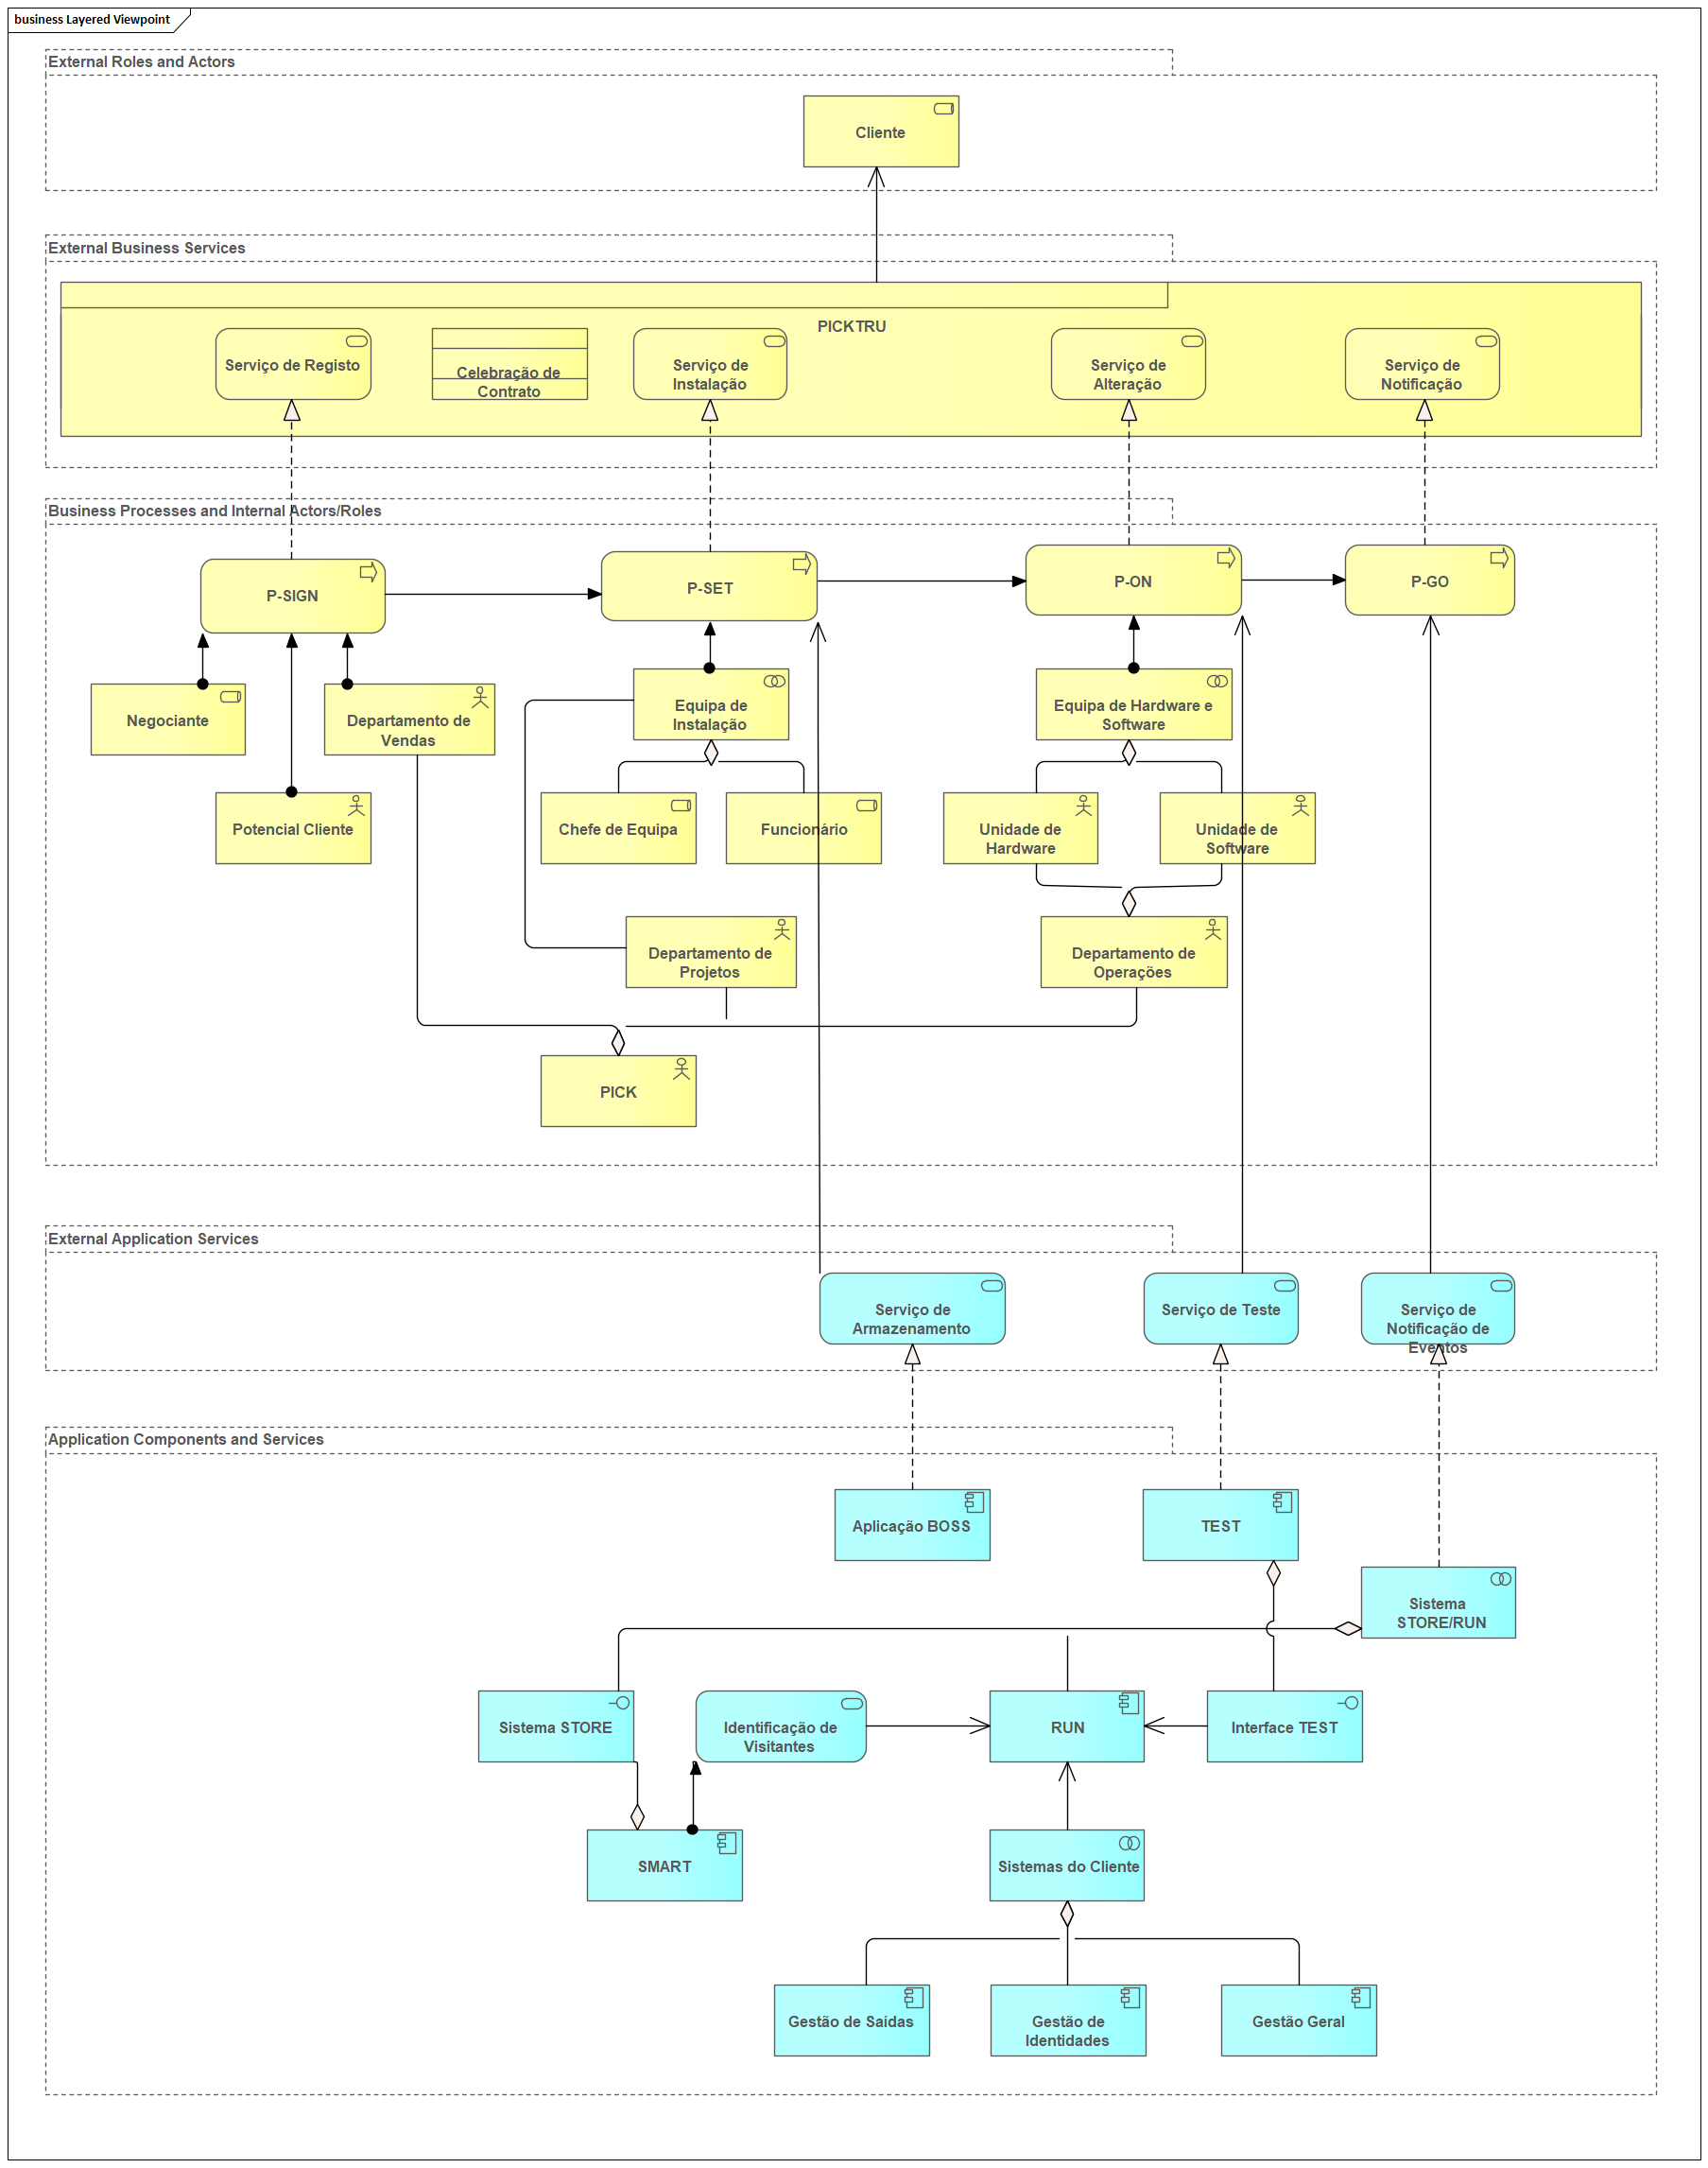
\includegraphics[width=\textwidth,height=\textheight,keepaspectratio]{A1-2}
\vspace*{\fill}

\pagebreak

\begin{landscape}
	\section*{A2 - Diagrama do Processo P-SET}
	\vspace*{\fill}
	\begin{center}
		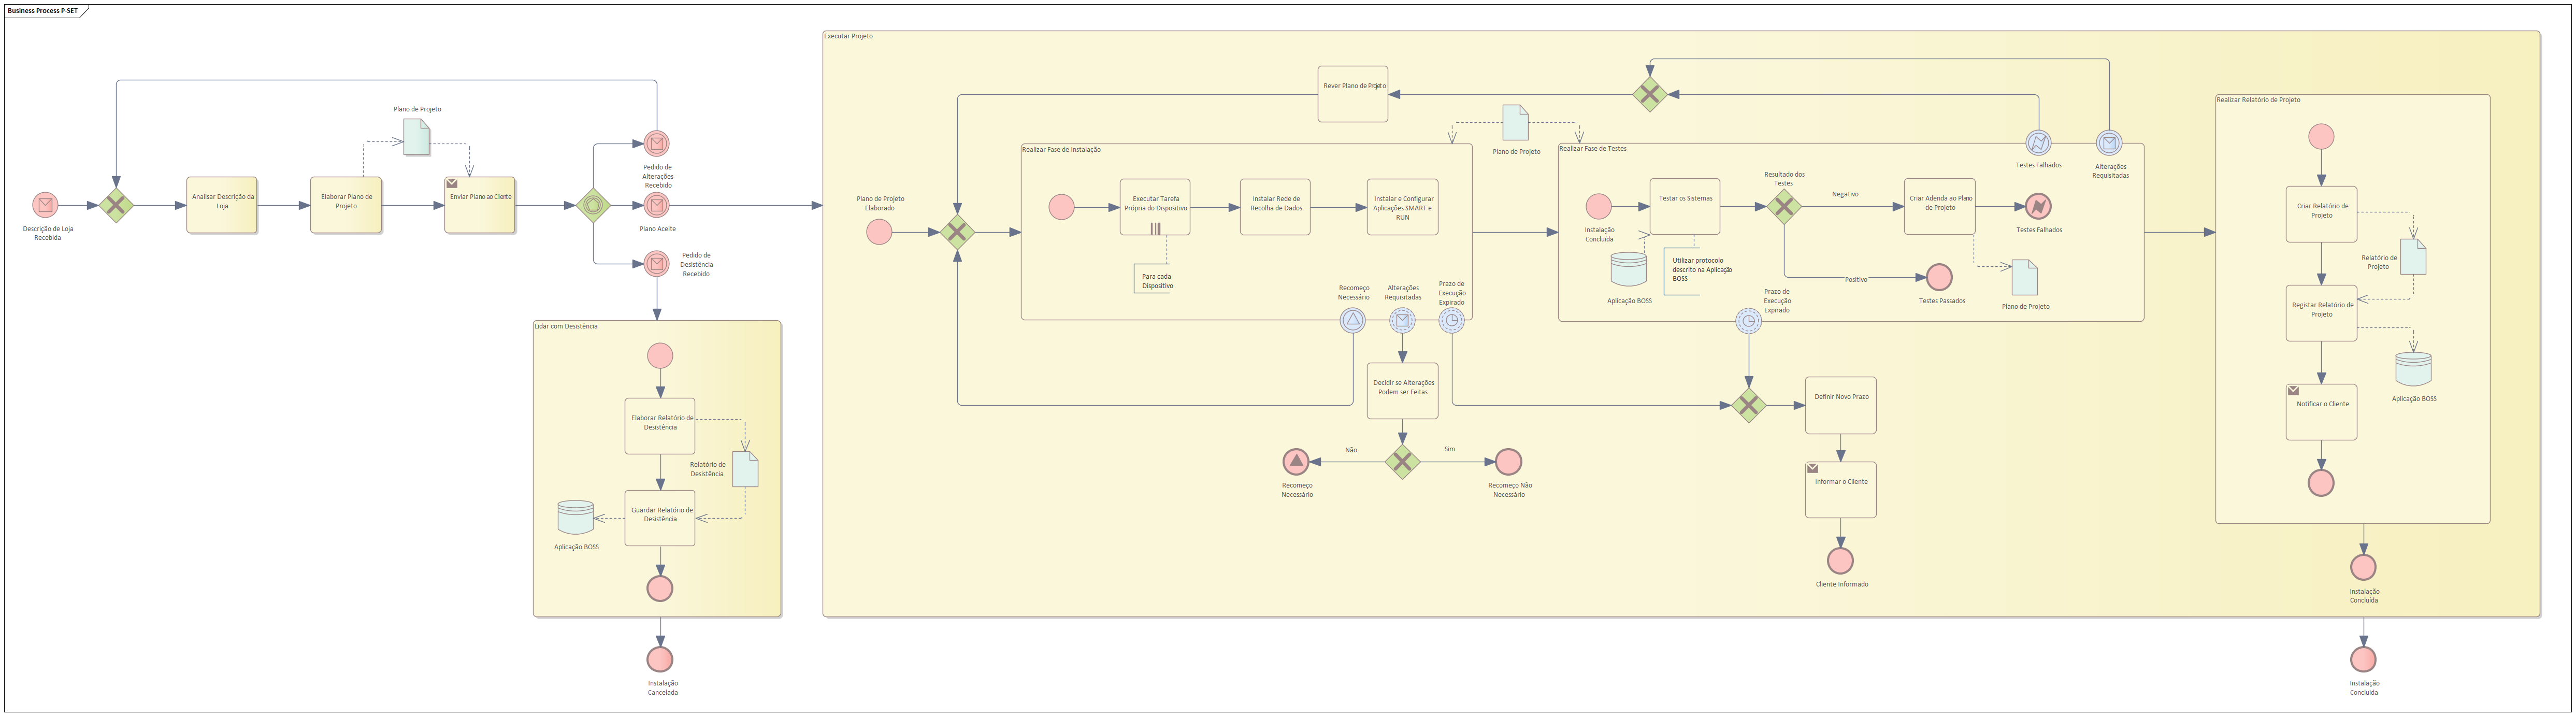
\includegraphics[width=1.5\textheight,height=\textwidth,keepaspectratio]{A2-2}
	\end{center}
	\vspace*{\fill}
\end{landscape}

\pagebreak

\begin{landscape}
	\section*{A3 - Diagrama do Processo P-ON}
	\vspace*{\fill}
	\begin{center}
		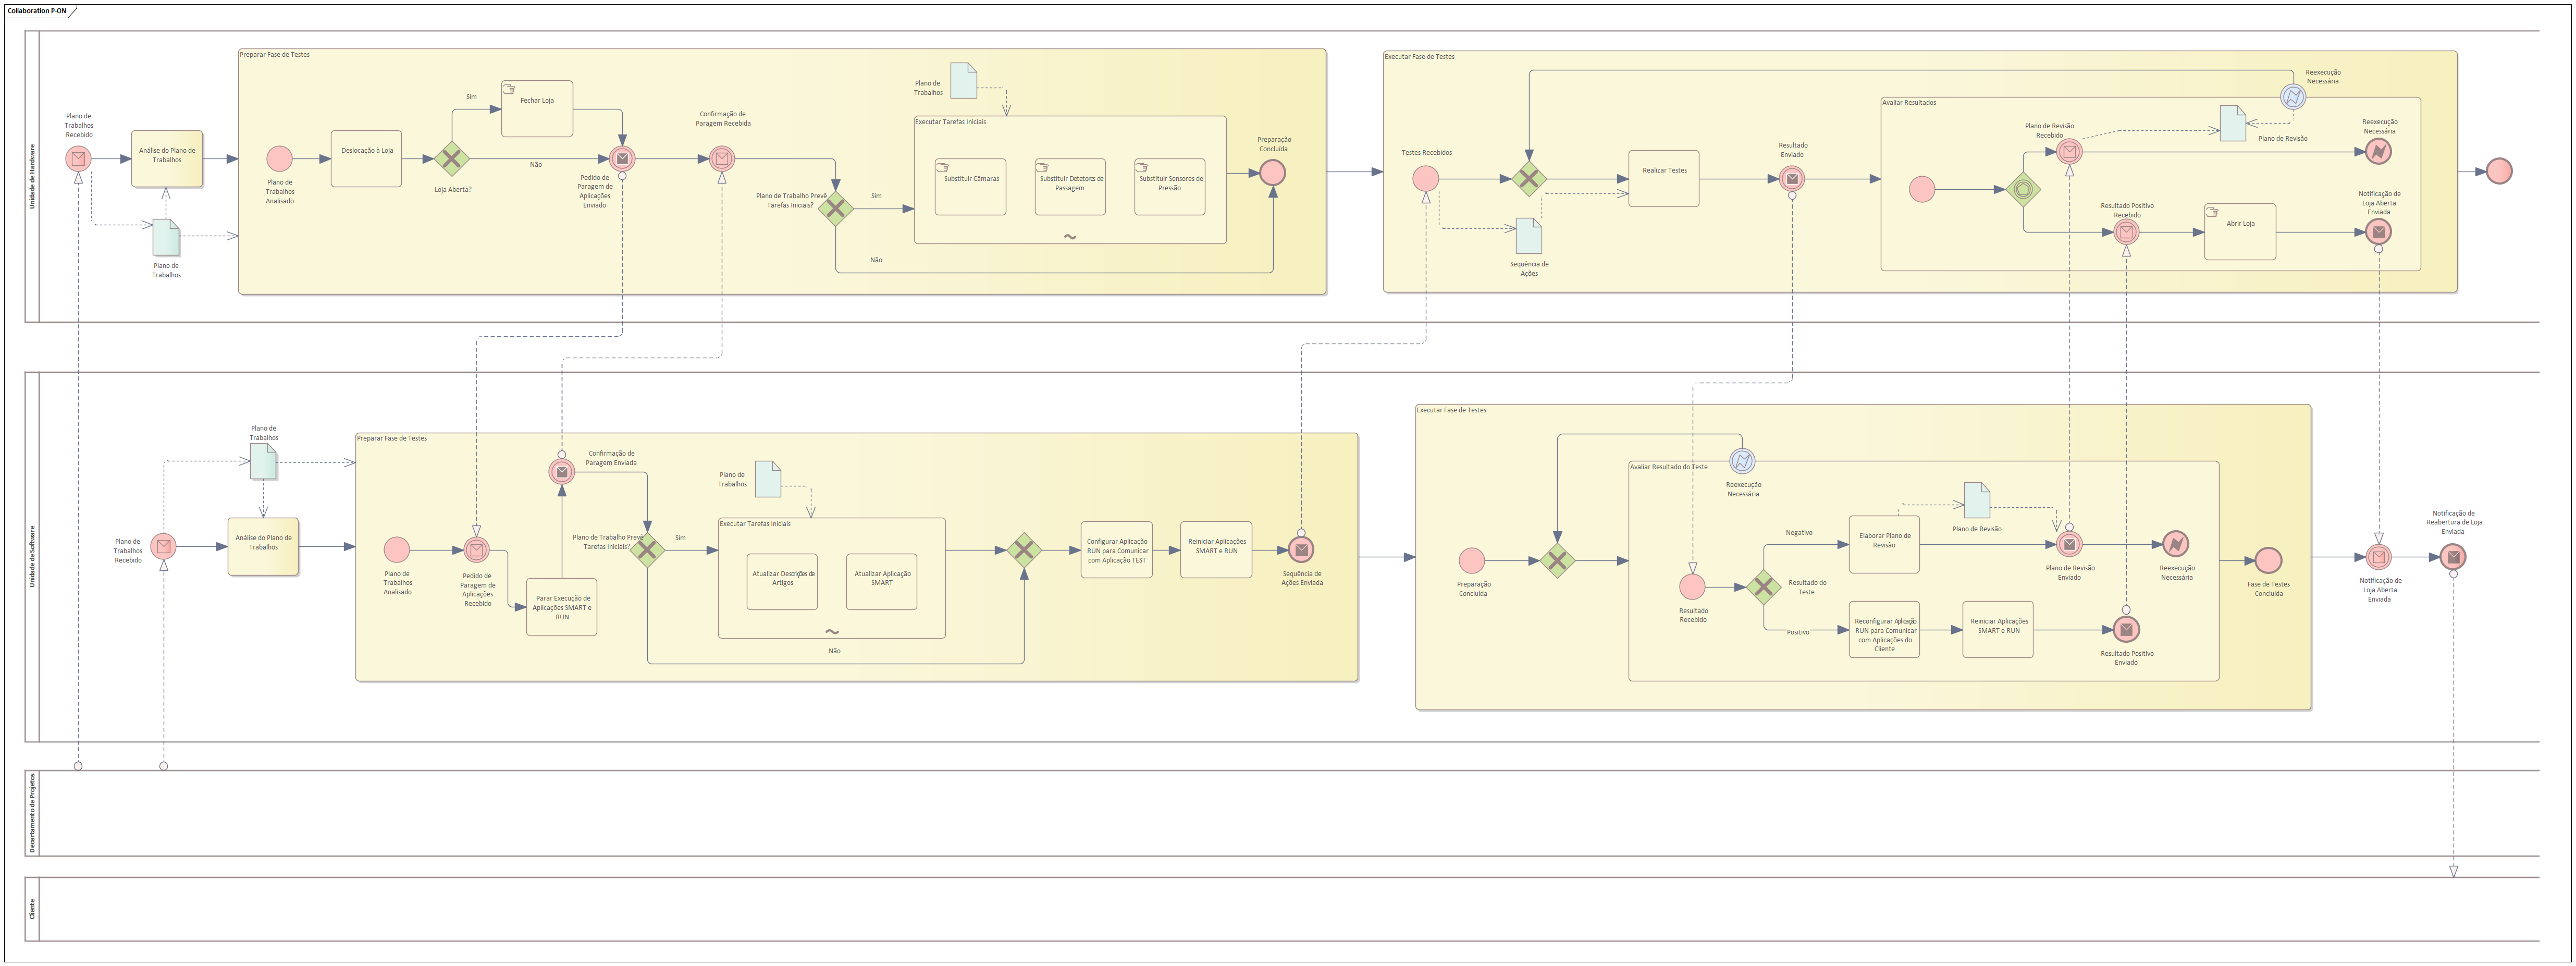
\includegraphics[width=1.5\textheight,height=\textwidth,keepaspectratio]{A3-2}
	\end{center}
	\vspace*{\fill}
\end{landscape}

\pagebreak

\section*{B2 - Diagrama de Casos de Uso - Sistema RUN}
\vspace*{\fill}
\begin{center}
	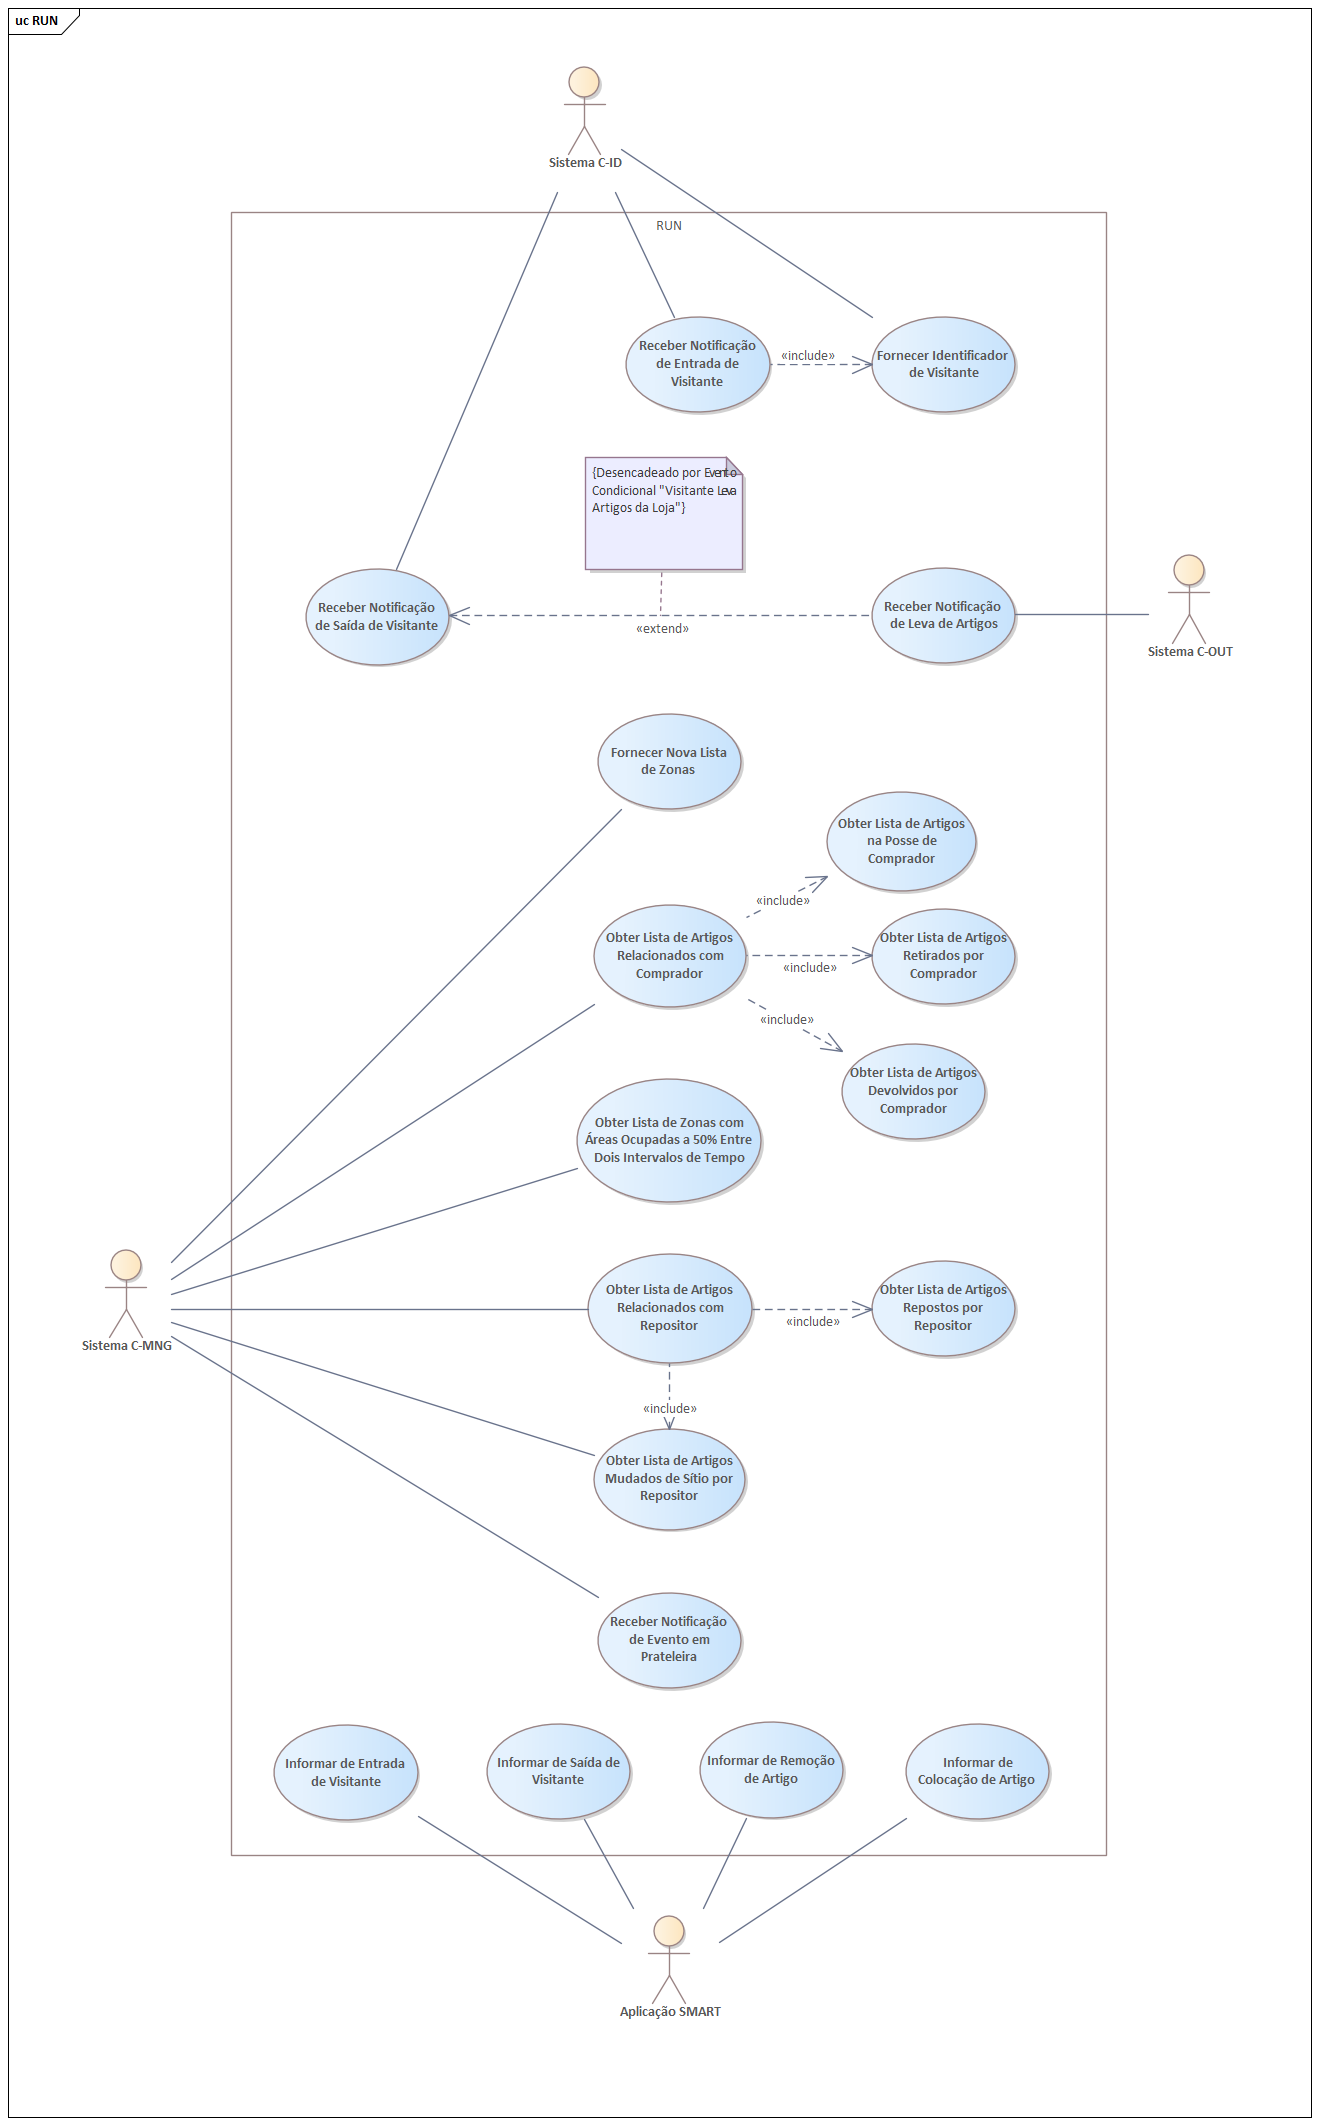
\includegraphics[width=0.95\textwidth,height=0.95\textheight,keepaspectratio]{B2-RUN}
\end{center}
\vspace*{\fill}

\pagebreak

\section*{B2 - Diagrama de Casos de Uso - Sistema STORE}
\vspace*{\fill}
\begin{center}
	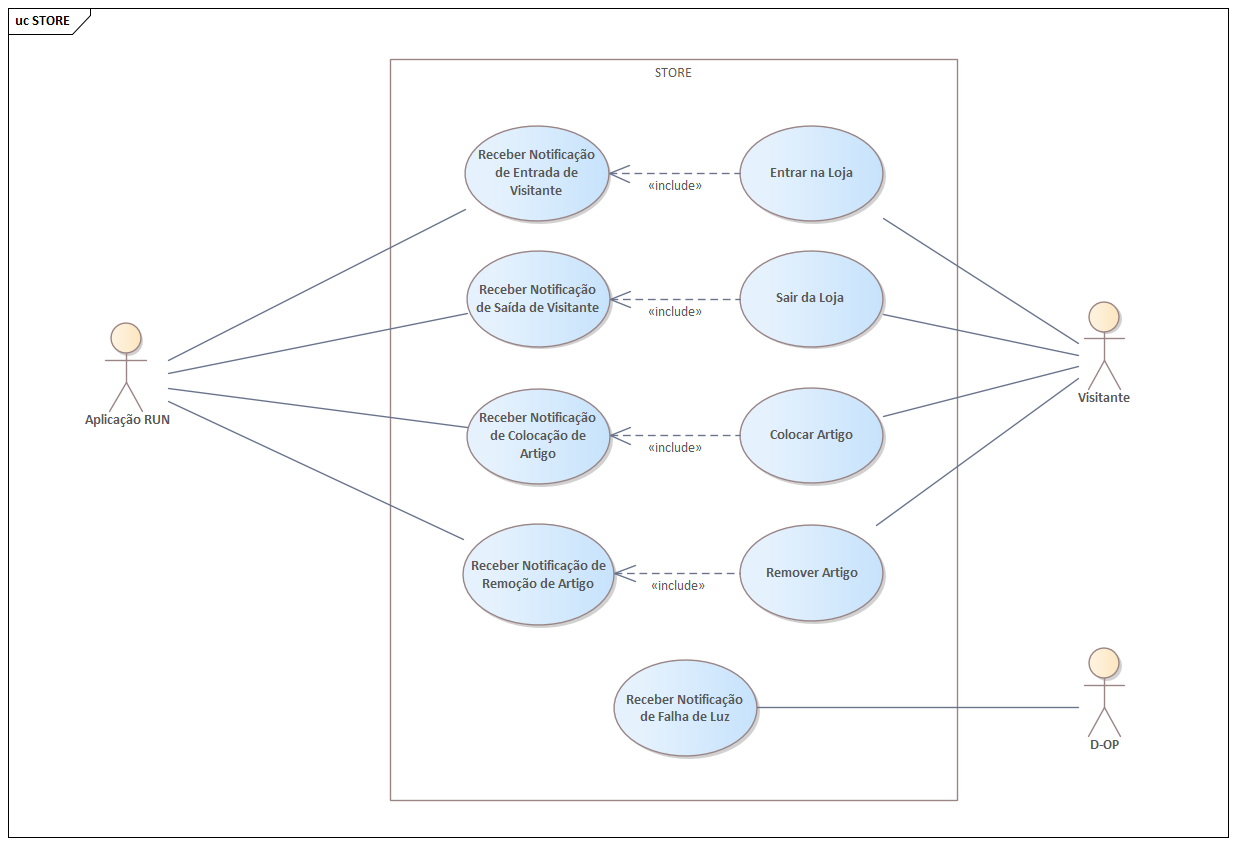
\includegraphics[width=\textwidth,height=\textheight,keepaspectratio]{B2-STORE}
\end{center}
\vspace*{\fill}

\pagebreak

\begin{landscape}
	\section*{B3 - Diagrama de Classes do Modelo de Domínio}
	\vspace*{\fill}
	\begin{center}
		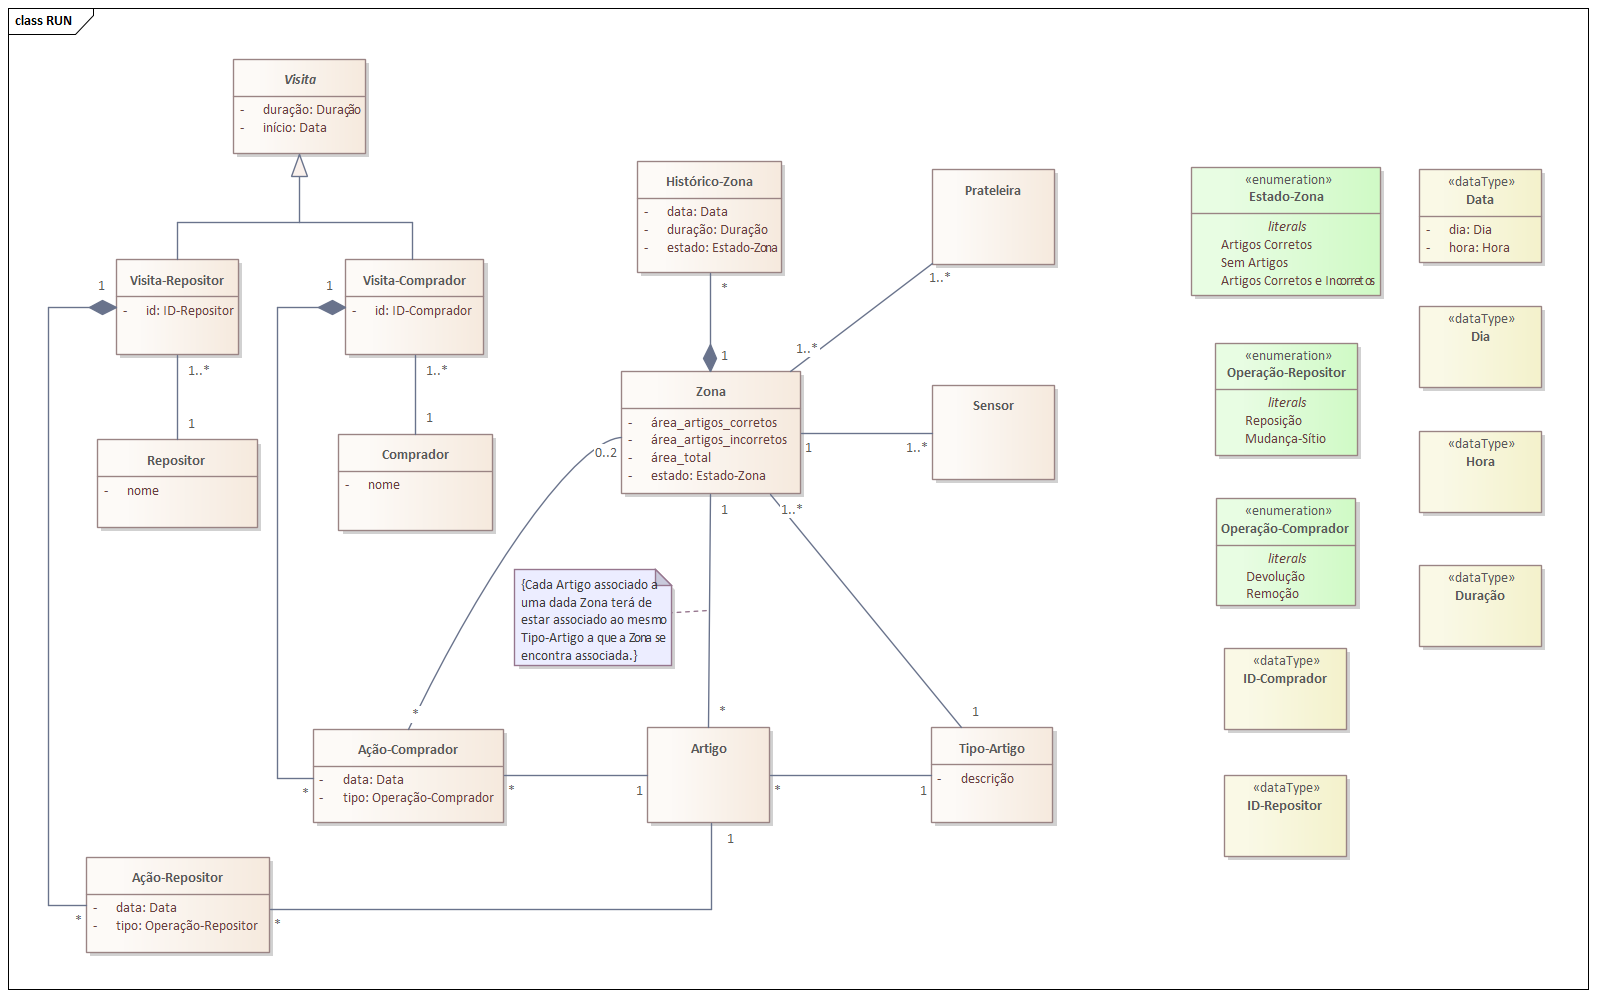
\includegraphics[width=1.45\textheight,height=\textwidth,keepaspectratio]{B3}
	\end{center}
	\vspace*{\fill}
\end{landscape}

\pagebreak

\begin{landscape}
	\section*{B4 - Diagrama de Máquina de Estados}
	\vspace*{\fill}
	\begin{center}
		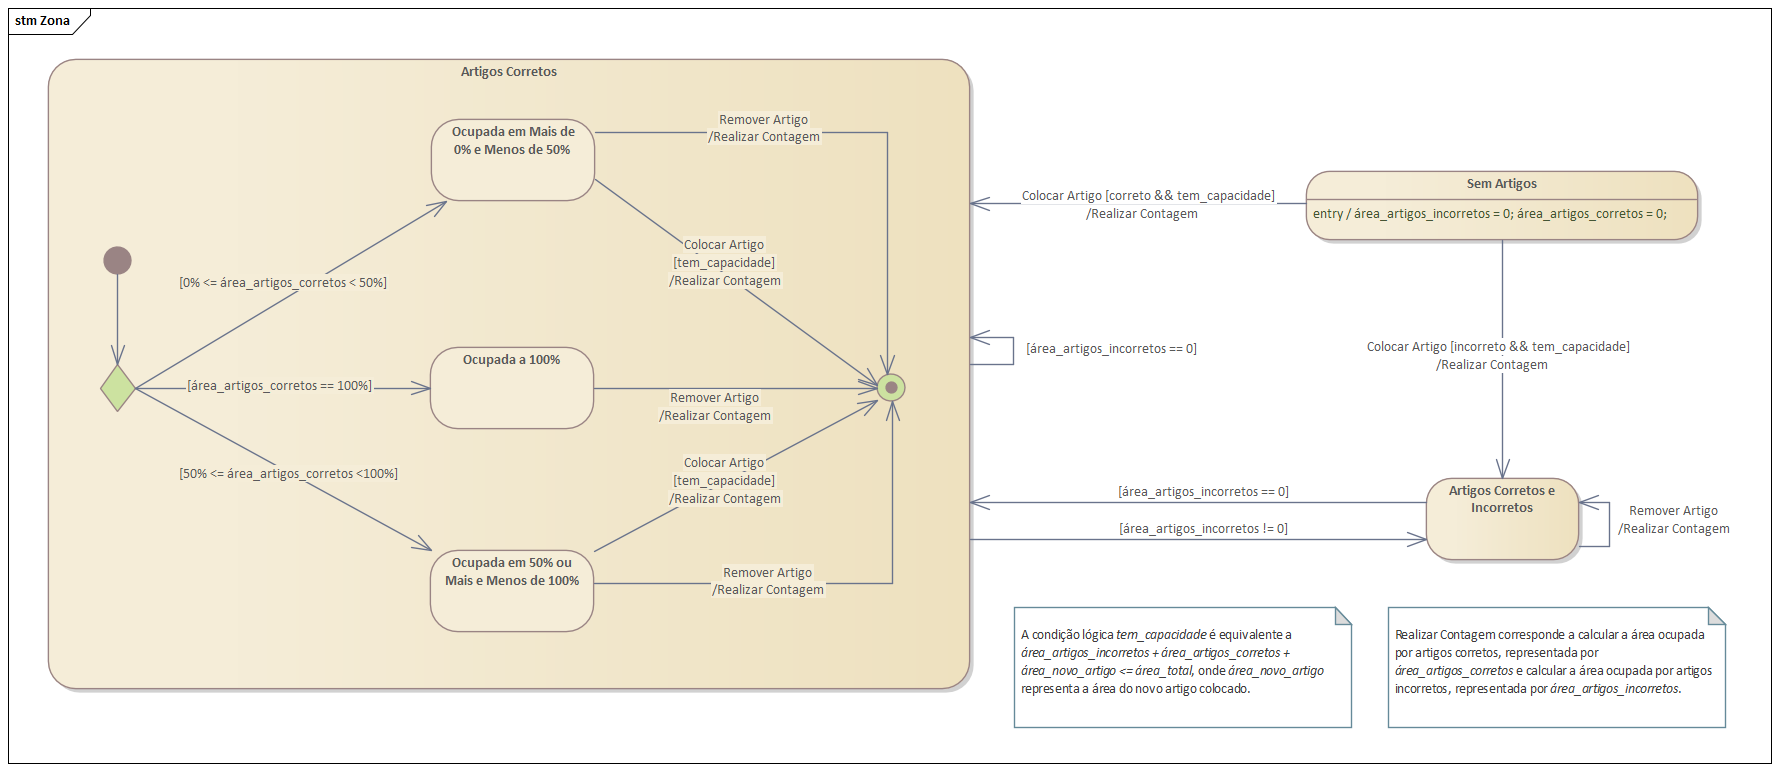
\includegraphics[width=1.5\textheight,height=\textwidth,keepaspectratio]{B4}
	\end{center}
	\vspace*{\fill}
\end{landscape}

\begin{landscape}
	\section*{B5 - Diagrama de Blocos}
	\vspace*{\fill}
	\begin{center}
		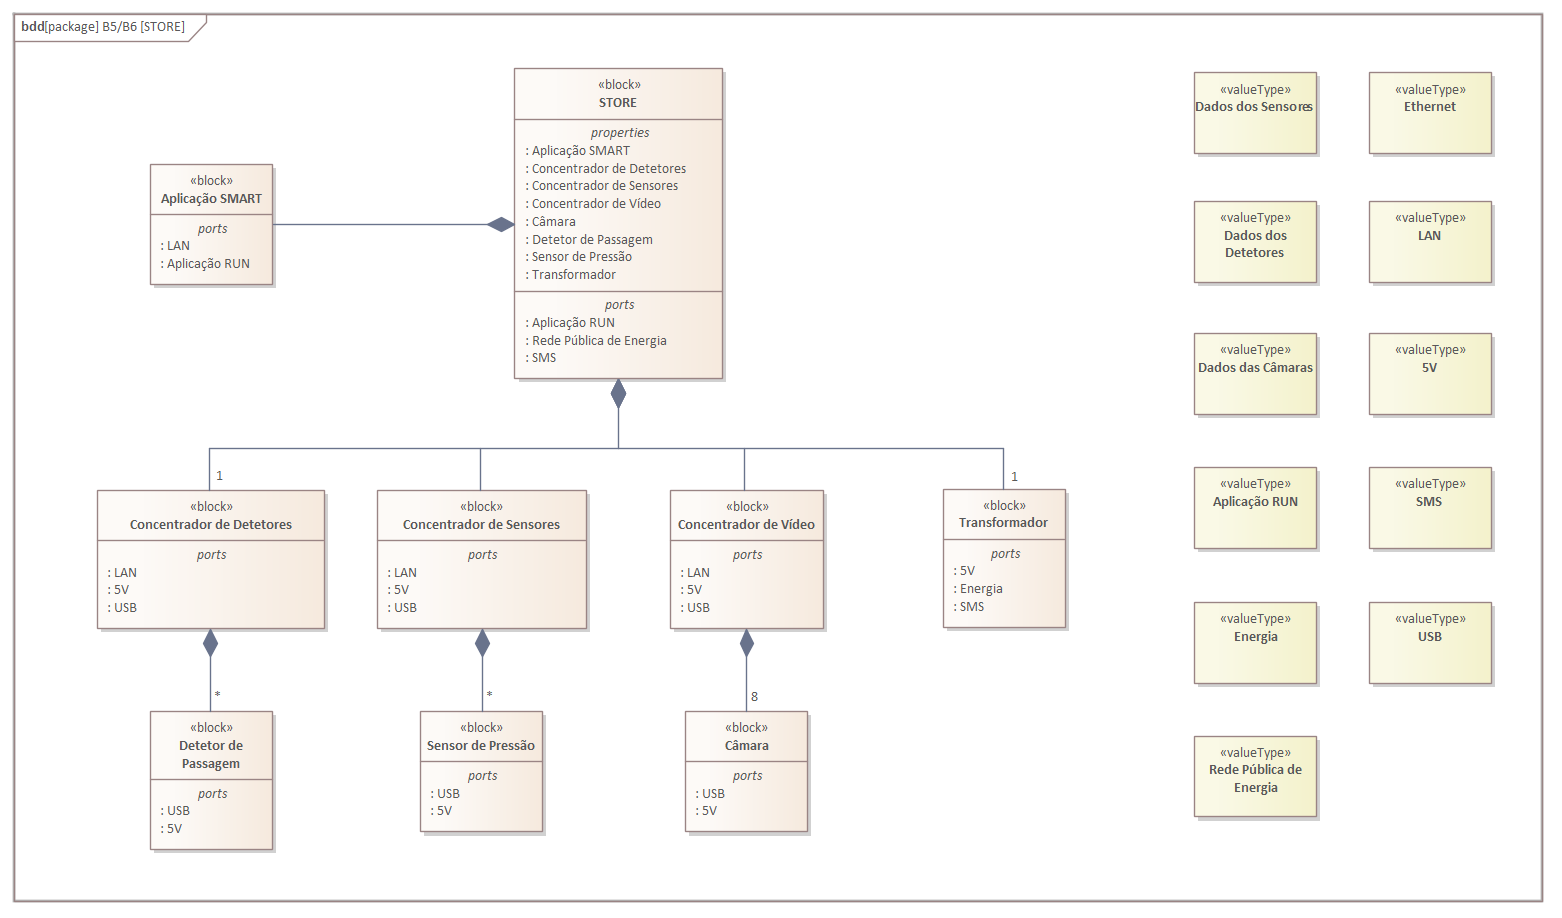
\includegraphics[width=1.5\textheight,height=\textwidth,keepaspectratio]{B5}
	\end{center}
	\vspace*{\fill}
\end{landscape}

\begin{landscape}
	\section*{B6 - Diagrama Interno de Blocos}
	\vspace*{\fill}
	\begin{center}
		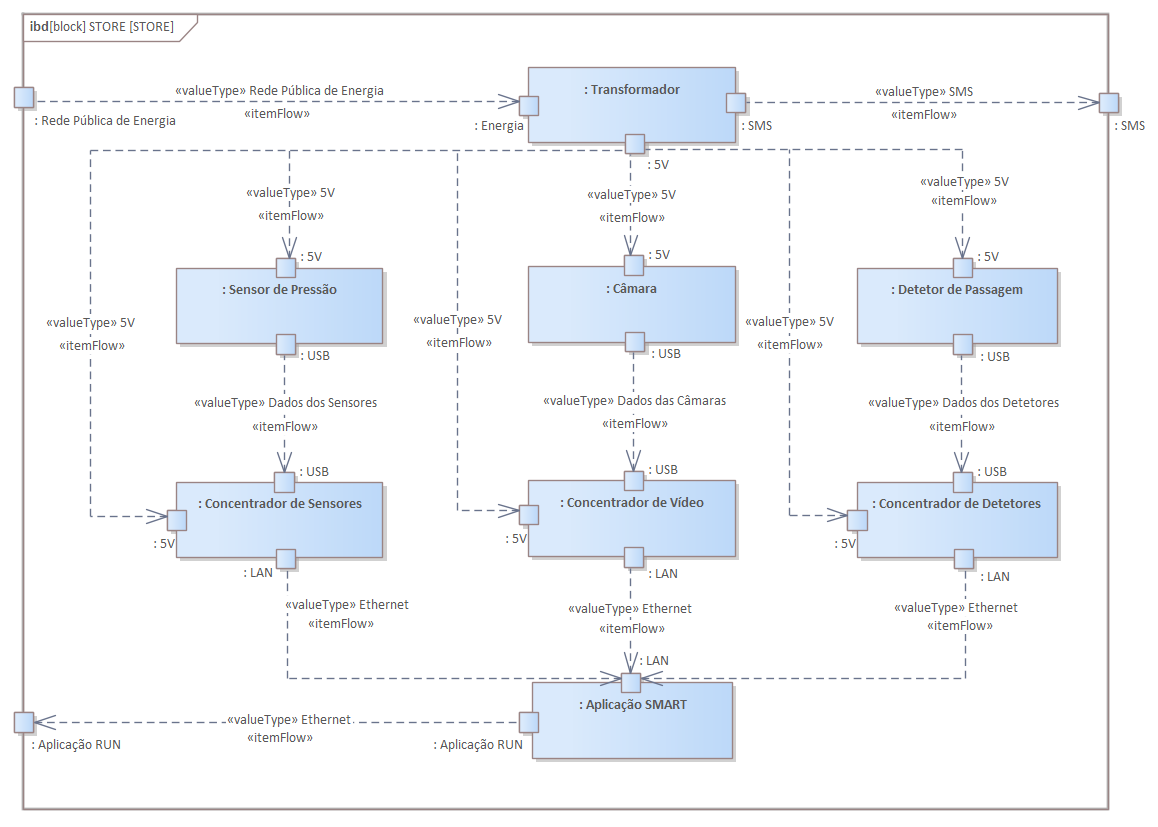
\includegraphics[width=1.3\textheight,height=\textwidth,keepaspectratio]{B6}
	\end{center}
	\vspace*{\fill}
\end{landscape}

\end{document}
